% JuliaCon proceedings template
\documentclass{juliacon}
%\usepackage{mathabx}
\usepackage{amsmath}
\usepackage{amssymb}
\usepackage{amsfonts}
\usepackage{lmodern}
\usepackage{fontawesome}
\usepackage{xcolor}
\definecolor{gray10}{gray}{0.95}
\usepackage{enumitem}

\usepackage{tikz}
\usetikzlibrary{shapes,arrows,calc}
\tikzstyle{block} = [thick, draw, rectangle, rounded corners, fill=blue!20,
                       minimum height=3em, minimum width=6em]
\tikzstyle{action} = [thick, draw, circle, fill=red!10]

\lstset{aboveskip=6pt,belowskip=6pt,frame=false,basicstyle=\ttfamily\small,language=Julia}

\newcommand{\R}{{\mathbb R}}
\newcommand{\N}{{\mathbb N}}
\newcommand{\E}{{\mathbb E}}
\newcommand{\Z}{{\mathbb Z}}
\renewcommand{\P}{{\mathbb P}}
\newcommand{\bbC}{{\mathbb C}}
\newcommand{\cO}{\mathcal{O}}
\newcommand{\cF}{\mathcal{F}}
\newcommand{\cE}{\mathcal{E}}
\newcommand{\cX}{\mathcal{X}}
\newcommand{\cA}{\mathcal{A}}
\newcommand{\cS}{\mathcal{S}}
\newcommand{\cR}{\mathcal{R}}
\newcommand{\cB}{\mathcal{B}}
\newcommand{\cP}{\mathcal{P}}
\newcommand{\cM}{\mathcal{M}}

\newcommand{\tV}{\widetilde{V}}
\newcommand{\tF}{\widetilde{F}}
\newcommand{\tQ}{\widetilde{Q}}

\newcommand{\bw}{\mathbold{w}}

\newcommand{\Inv}{\mathop{\mathrm{Inv}}}
\newcommand{\argmax}{\mathop{\mathrm{argmax}}}
\newcommand{\mean}{\mathop{\mathrm{mean}}}
\newcommand{\diam}{\mathop{\mathrm{diam}}}

\newcommand{\todo}[1]{\textcolor{red}{\texttt{#1}}}

\setcounter{page}{1}

\begin{document}

% **************GENERATED FILE, DO NOT EDIT**************

\title{Fast, Elegant, Set-oriented Numerical Analysis using GAIO.jl}

\author[1]{A. Herwig}
\author[1]{O. Junge}
\affil[1]{Technical University Munich}

\keywords{Dynamical Systems}

\hypersetup{
pdftitle = {Fast, Elegant, Set-oriented Numerical Analysis using GAIO.jl},
pdfsubject = {JuliaCon 2022 Proceedings},
pdfauthor = {A. Herwig, O. Junge},
pdfkeywords = {Dynamical Systems},
}



\maketitle

\vfill

\begin{abstract}

We provide an implementation of set-oriented numerical methods \cite{DeJu:02,DeFrJu:01} in a Julia package. In the context of dynamical systems, the package enables the rigorous computation of invariant sets (e.g. chain recurrent sets, attractors and invariant manifolds) and provides discretizations of the transfer and the Koopman operator, enabling the computation of, e.g., invariant measures, almost invariant, cyclic and coherent sets. The redesign of the original implementation \cite{GAIO} in Julia presented in this note has a more concise syntax, while showing the same or even better performance.

\end{abstract}

\section{Introduction}

This note presents an implementation of a \emph{set-oriented} approach  to numerical computations approach \cite{DeJu:02,DeFrJu:01} in the Julia language, encapsulated in the package GAIO.jl. The data structures and the algorithmic interface have been completely redesigned over the original implementation in C \cite{GAIO}. As a result, the code for the set-oriented algorithms is very concise and close to its mathematical pseudocode. At the same time, the performance is equal or better. We showcase the features of GAIO.jl by some classical computations of invariant sets and (almost) invariant measures in dynamical systems.  

A \emph{dynamical system} is a mathematical model of a system whose state evolves with time.  Key questions about the possible evolutions in a system  include whether certain subsets of state space are invariant, the stability of these subsets as well as questions about statistical properties of typical trajectories. Such topological and statistical questions (among others) can be answered using set-oriented numerical techniques \cite{DeJu:02,DeFrJu:01}, see also \cite{Hsu:13,Mi:02}. 

We give a brief introduction on what can be computed with GAIO.jl in Section~\ref{sec:computations} and then talk about the architecture of the package in Section~\ref{sec:architecture}.

%\eject

\section{Global Analysis of Dynamical Systems}
\label{sec:computations}

A dynamical system in which time is modelled in discrete steps is given by a map $f : X \to X$ on some domain $X$. We assume $X$ to be a compact subset of $\R^d$ and $f$ to be a homeomorphism, i.e.\ bijective, continuous with a continuous inverse. We recall some basic notions from dynamical systems literature required for the proceeding example. 

\subsection{Geometric/topological analysis}\label{sec:attractors}

A set $Y \subset X$ is \emph{forward invariant} if $f(Y) \subset Y$, \emph{backward invariant} if $f^{-1}(Y) \subset Y$ \footnote{$f^{-1}(Y)$ denotes the preimage of the set $Y$}, and \emph{invariant} if it is both forward and backward invariant. An invariant set is called \emph{attracting} if there exists a neighborhood $U \supset Y$ such that for any other neighborhood $V \supset Y$ there exists a $k_0 \in \N$ such that $f^k (U) \subset V$ for all $k\geq k_0$. 

The \emph{maximal invariant set} contained in $Y$ is the set 
    \begin{equation}
        \Inv (Y) = \left\{ x \in Y \mid f^k(x) \in Y \text{ for all } k\in\Z \right\}.
    \end{equation}

It follows immediately from the definition that $\Inv (Y)$ contains all other invariant sets which are contained in $Y$. The following proposition is important for its computation. 

\begin{proposition}
    \cite{maxinvset}
    If $Y \subset X$ is forward invariant, then $\Inv (Y) = \bigcap_{k \geq 0} f^k (Y)$. 
\end{proposition}

If $Y$ is not forward invariant, the set $A_Y=\bigcap_{k \geq 0} f^k (A)$ is called the \emph{attractor relative to $Y$} \cite{DeHo:97}. The proposition leads to a natural ansatz for approximation by repeatedly tightening a cover of the set by finite collections of sets \cite{DeHo:97}. Specifically, given a partition $\cP$ of $X$ into (essentially) disjoint sets and a covering $\cB$ of $A_Y$ by elements of $\cP$, repeat the following two steps until a prescribed diameter of the partition elements is reached:

\begin{enumerate}
    \item Refine $\cP$ into a strictly finer partition $\cP'$ such that $\diam (\cP') \leq \theta \cdot \diam (\cP)$ for some fixed $\theta < 1$. Let $\cB'$ be the (refined) covering $\cB$. 
    \item Map the covering forward under $f$, i.e. cover\footnote{$\vert \cB \vert = \bigcup_{B \in \cB} B$} $f(\vert\cB'\vert)$  by elements of $\cP$. Intersect this covering with $\cB'$. 
\end{enumerate}

A simple way to partition a \emph{box} $$X = \left[ \ell_1, u_1 \right] \times \ldots \times \left[ \ell_d, u_d \right]$$  is to divide it into an $n_1 \times \ldots \times n_d$ - element grid of boxes. 

\subsubsection*{Example: A four wing attractor}

Consider the ordinary differential equation \cite{3dattractor}
\begin{equation}
    \label{eq:ode}
    \begin{split}
        &\dot{x} = ax + yz \\
        &\dot{y} = dy + bx - zy \\ 
        &\dot{z} = -z - xy 
    \end{split}
\end{equation}
where $a,b,d \in \R$ are parameters. Let $f$ be the time-$2$ flow map of the system, discretized using 20 steps of the standard Runge-Kutta $4$th order method:
\begin{lstlisting}[language=Julia,label=lst:map,backgroundcolor=\color{gray10},mathescape]
const a, b, d = 0$\texttt{.2}$, -0$\texttt{.0}$1, -0$\texttt{.4}$
v((x,y,z)) = @. (a*x+y*z, d*y+b*x-z*y, -z-x*y)
f(x) = rk4_flow_map(v, x, 0$\texttt{.0}$1, 20)
\end{lstlisting}
\begin{lstlisting}[language=Julia,backgroundcolor=\color{gray10},mathescape]
# illustrative initial condition
x0 = (0$\texttt{.9}$4, -2$\texttt{.2}$, 0$\texttt{.4}$)
trajectory = [x0]
for _ in 1:100_000
    x = trajectory[end]
    push!(trajectory, f(x))
end
lines(trajectory)
\end{lstlisting}
Figure~\ref{fig:trajectories} shows the resulting trajectory.  Of course, any other package for solving initial value problems (e.g.\ from DifferentialEquations.jl or DynamicalSystems.jl) can be used in order to approximate the flow map. Note, however, that we will need to evaluate $f$ on many initial conditions so efficiency of the solver matters.
\begin{figure}[h]
    \centering
    \includegraphics[width=0.45\textwidth]{trajectories.png}
    \caption{A trajectory of the four wing system.}
    \label{fig:trajectories}
\end{figure}

We now compute a covering of the attractor of the system.  To this end, we first construct a partition $\cP$ of the domain $X = \left[ -5, 5 \right]^3$ into a $2 \times 2 \times 2$ grid of boxes: 
\begin{lstlisting}[label=lst:box,backgroundcolor=\color{gray10}]
center = (0., 0., 0.)
radius = (5., 5., 5.)
X = Box(center, radius)
P = BoxPartition(X, (2, 2, 2))
\end{lstlisting}

The flow map $f$ induces a map\footnote{For some set $S$, $2^S$ denotes the power set of $S$.} $F : 2^\cP \to 2^\cP$ by the relationship 
\begin{equation}
    F \left( \left\{ B \right\} \right) = 
    %\bigcup_{\substack{
    %    C \in \cP \\ C \cap f(B) \neq \emptyset
    %}} \left\{ C\right\}
    \left\{ C \in \cP \mid C \cap f(B) \neq \emptyset \right\}
\end{equation}
%
as sketched in Fig. \ref{fig:boxcover}. 
%
\begin{figure}[h]
    \centering
    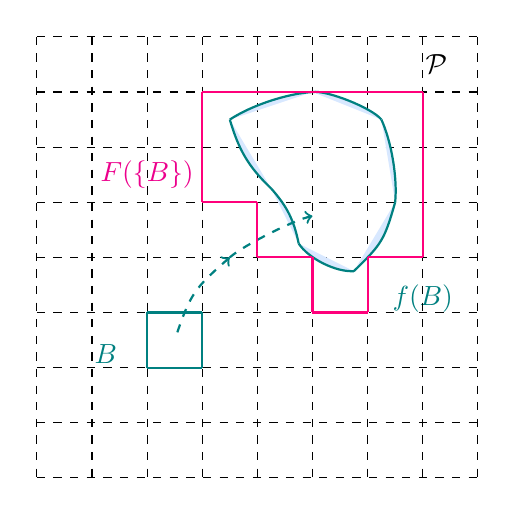
\begin{tikzpicture}[scale=0.7]
    \node [color=black] (0) at (-4, 4) {};
    \node [color=black] (1) at (-3, 4) {};
    \node [color=black] (2) at (-2, 4) {};
    \node [color=black] (3) at (-1, 4) {};
    \node [color=black] (4) at (0, 4) {};
    \node [color=black] (5) at (1, 4) {};
    \node [color=black] (6) at (2, 4) {};
    \node [color=black] (7) at (3, 4) {};
    \node [color=black] (8) at (4, 4) {};
    \node [color=black] (9) at (4, 3) {};
    \node [color=black] (10) at (4, 2) {};
    \node [color=black] (11) at (4, 1) {};
    \node [color=black] (12) at (4, 0) {};
    \node [color=black] (13) at (4, -1) {};
    \node [color=black] (14) at (4, -2) {};
    \node [color=black] (15) at (4, -3) {};
    \node [color=black] (16) at (4, -4) {};
    \node [color=black] (17) at (3, -4) {};
    \node [color=black] (18) at (2, -4) {};
    \node [color=black] (19) at (1, -4) {};
    \node [color=black] (20) at (0, -4) {};
    \node [color=black] (21) at (-1, -4) {};
    \node [color=black] (22) at (-2, -4) {};
    \node [color=black] (23) at (-3, -4) {};
    \node [color=black] (24) at (-4, -4) {};
    \node [color=black] (25) at (-4, -3) {};
    \node [color=black] (26) at (-4, -2) {};
    \node [color=black] (27) at (-4, -1) {};
    \node [color=black] (28) at (-4, 0) {};
    \node [color=black] (29) at (-4, 1) {};
    \node [color=black] (30) at (-4, 2) {};
    \node [color=black] (31) at (-4, 3) {};
    \node [color=black] (32) at (-2, -1) {};
    \node [color=black] (33) at (-1, -1) {};
    \node [color=black] (34) at (-1, -2) {};
    \node [color=black] (35) at (-2, -2) {};
    \node [color=black] (36) at (-2.75, -1.75) {\textcolor{teal}{$B$}};
    \node [color=black] (37) at (-1.5, -1.5) {};
    \node [color=black] (38) at (-0.5, 2.5) {};
    \node [color=black] (39) at (0.25, 1.25) {};
    \node [color=black] (40) at (0.75, 0.25) {};
    \node [color=black] (41) at (1.75, -0.25) {};
    \node [color=black] (42) at (2.5, 1) {};
    \node [color=black] (43) at (2.25, 2.5) {};
    \node [color=black] (44) at (1, 3) {};
    \node [color=black] (45) at (3, -0.75) {\textcolor{teal}{$f(B)$}};
    \node [color=black] (46) at (1, 0.75) {};
    \node [color=black] (47) at (-0.5, 0) {};
    \node [color=black] (48) at (-1, 3) {};
    \node [color=black] (49) at (3, 3) {};
    \node [color=black] (50) at (3, 0) {};
    \node [color=black] (51) at (0, 0) {};
    \node [color=black] (52) at (0, 1) {};
    \node [color=black] (53) at (-1, 1) {};
    \node [color=black] (54) at (2, 0) {};
    \node [color=black] (55) at (1, 0) {};
    \node [color=black] (56) at (1, -1) {};
    \node [color=black] (57) at (2, -1) {};
    \node [color=black] (58) at (-2, 1.5) {};
    \node [color=black] (59) at (-2, 1.5) {\textcolor{magenta}{$F(\{ B \})$}};
    \node [color=black] (60) at (3.25, 3.5) {$\mathcal{P}$};

    \draw [-, dashed] (0.center) to (24.center);
    \draw [-, dashed] (1.center) to (23.center);
    \draw [-, dashed] (2.center) to (22.center);
    \draw [-, dashed] (3.center) to (21.center);
    \draw [-, dashed] (4.center) to (20.center);
    \draw [-, dashed] (5.center) to (19.center);
    \draw [-, dashed] (6.center) to (18.center);
    \draw [-, dashed] (7.center) to (17.center);
    \draw [-, dashed] (8.center) to (16.center);
    \draw [-, dashed] (0.center) to (8.center);
    \draw [-, dashed] (31.center) to (9.center);
    \draw [-, dashed] (30.center) to (10.center);
    \draw [-, dashed] (29.center) to (11.center);
    \draw [-, dashed] (28.center) to (12.center);
    \draw [-, dashed] (27.center) to (13.center);
    \draw [-, dashed] (26.center) to (14.center);
    \draw [-, dashed] (25.center) to (15.center);
    \draw [-, dashed] (24.center) to (16.center);
    \draw [-, draw={rgb,255: red,0; green,128; blue,128}, fill={rgb,255: red,216; green,232; blue,255}, thick] (32.center) to (33.center);
    \draw [-, draw={rgb,255: red,0; green,128; blue,128}, fill={rgb,255: red,216; green,232; blue,255}, thick] (33.center) to (34.center);
    \draw [-, draw={rgb,255: red,0; green,128; blue,128}, fill={rgb,255: red,216; green,232; blue,255}, thick] (34.center) to (35.center);
    \draw [-, draw={rgb,255: red,0; green,128; blue,128}, fill={rgb,255: red,216; green,232; blue,255}, thick] (35.center) to (32.center);
    \draw [-, draw={rgb,255: red,0; green,128; blue,128}, fill={rgb,255: red,216; green,232; blue,255}, thick, bend right=15] (38.center) to (39.center);
    \draw [-, draw={rgb,255: red,0; green,128; blue,128}, fill={rgb,255: red,216; green,232; blue,255}, thick, bend left=15] (39.center) to (40.center);
    \draw [-, draw={rgb,255: red,0; green,128; blue,128}, fill={rgb,255: red,216; green,232; blue,255}, thick, bend right, looseness=0.75] (40.center) to (41.center);
    \draw [-, draw={rgb,255: red,0; green,128; blue,128}, fill={rgb,255: red,216; green,232; blue,255}, thick, bend right=15, looseness=1.25] (41.center) to (42.center);
    \draw [-, draw={rgb,255: red,0; green,128; blue,128}, fill={rgb,255: red,216; green,232; blue,255}, thick, bend right=15, looseness=0.75] (42.center) to (43.center);
    \draw [-, draw={rgb,255: red,0; green,128; blue,128}, fill={rgb,255: red,216; green,232; blue,255}, thick, bend right, looseness=0.50] (43.center) to (44.center);
    \draw [-, draw={rgb,255: red,0; green,128; blue,128}, fill={rgb,255: red,216; green,232; blue,255}, thick, bend right=15, looseness=0.75] (44.center) to (38.center);
    \draw [fill=none, draw={rgb,255: red,0; green,128; blue,128}, dashed, <-, thick, bend right=15, looseness=1.25] (47.center) to (37.center);
    \draw [fill=none, draw={rgb,255: red,0; green,128; blue,128}, dashed, <-, thick, bend right=15, looseness=0.50] (46.center) to (47.center);
    \draw [-, draw={rgb,255: red,255; green,0; blue,123}, fill={rgb,255: red,255; green,221; blue,228}, thick] (51.center) to (52.center);
    \draw [-, draw={rgb,255: red,255; green,0; blue,123}, fill={rgb,255: red,255; green,221; blue,228}, thick] (52.center) to (53.center);
    \draw [-, draw={rgb,255: red,255; green,0; blue,123}, fill={rgb,255: red,255; green,221; blue,228}, thick] (53.center) to (48.center);
    \draw [-, draw={rgb,255: red,255; green,0; blue,123}, fill={rgb,255: red,255; green,221; blue,228}, thick] (48.center) to (49.center);
    \draw [-, draw={rgb,255: red,255; green,0; blue,123}, fill={rgb,255: red,255; green,221; blue,228}, thick] (49.center) to (50.center);
    \draw [-, draw={rgb,255: red,255; green,0; blue,123}, fill={rgb,255: red,255; green,221; blue,228}, thick] (50.center) to (54.center);
    \draw [-, draw={rgb,255: red,255; green,0; blue,123}, fill={rgb,255: red,255; green,221; blue,228}, thick] (54.center) to (57.center);
    \draw [-, draw={rgb,255: red,255; green,0; blue,123}, fill={rgb,255: red,255; green,221; blue,228}, thick] (57.center) to (56.center);
    \draw [-, draw={rgb,255: red,255; green,0; blue,123}, fill={rgb,255: red,255; green,221; blue,228}, thick] (56.center) to (55.center);
    \draw [-, draw={rgb,255: red,255; green,0; blue,123}, fill={rgb,255: red,255; green,221; blue,228}, thick] (55.center) to (51.center);
\end{tikzpicture}

    \caption{The map $f:X\to X$ induces a map $F : 2^\cP \to 2^\cP$.}
    \label{fig:boxcover}
\end{figure}
%
GAIO.jl provides multiple methods for approximating the map $F$. An intuitive method is to sample some points  uniformly within a box, and then map each point with $f$:  
\begin{lstlisting}[backgroundcolor=\color{gray10}]
F = BoxMap(:montecarlo, f, Q)
\end{lstlisting}
If a rigorous (outer) cover of the image $F(\{B\})$ is required, special sampling techniques \cite{rigoroussampling} and/or interval arithmetic can be used.
We can now implement the above algorithm as shown in Figure~\ref{fig:attr_julia}.  In each iteration we cycle through the coordinate direction in which we bisect the boxes of the current covering.
\begin{figure}[h]
\begin{lstlisting}[language=Julia,backgroundcolor=\color{gray10},mathescape]
function relative_attractor(F, B; steps)
    for k in 1:steps
        B = subdivide(B, k % 3 + 1)
        B = F(B) $\cap$ B
    end
    return $B$
end
\end{lstlisting}
\caption{Implementation if the subdivison algorithm in GAIO.jl. Compare with the implementation in Fig. \ref{fig:attr_matlab}.}
\label{fig:attr_julia}
\end{figure}

In order to invoke this function, we first construct the initial covering by collecting all boxes from the partition:
\begin{lstlisting}[language=Julia,mathescape,backgroundcolor=\color{gray10}]
B = cover(P, :)
A = relative_attractor(F, B, steps=21)
plot(A)
\end{lstlisting}

The computed covering of the attractor relative to $X$ is shown in Fig. \ref{fig:attractor}.  

\begin{figure}[h]
    \centering
    \includegraphics[width=0.45\textwidth]{attractor.png}
    \caption{Computed relative attractor of the system described in Eq. \ref{eq:ode}}
    \label{fig:attractor}
\end{figure}


Other algorithms implemented in GAIO.jl include ones for computing
\begin{itemize}[label=$\bullet$]
    \item forward, backward and maximal invariant sets,
    \item (un-)stable manifolds,
    \item chain-recurrent sets,
    \item Morse decompositions.
\end{itemize}

\subsection{Statistical analysis}
\label{sec:architecture}

The map $f:X \to X$ induces a map $f_\sharp : \cM \to \cM$ on measures\footnote{$\cM$ denotes the space of finite, complex valued Borel measures on $X$} via 
\begin{equation}
    f_\sharp\, \mu := \mu \circ f^{-1}.
\end{equation}
This is a bounded linear Markov operator, the \emph{Perron-Frobenius} or \emph{transfer operator}.  A lot of information about macroscopic features of the dynamics of $f$ can be extracted from eigenmeasures of $f_\sharp$ at eigenvalues with modulus close to one \cite{DeJu:99}.   

In particular, there exists \cite{invariantmeasureexistence} an eigenmeasure $\mu = f_\sharp\, \mu$ at the eigenvalue $1$ of $f_\sharp$, an \emph{invariant measure}. A \emph{natural} invariant measure \cite{} quantifies the statistics of typical trajectories: regions of phase space which are visited more often by such trajectories receive more $\mu$-mass.  

\subsubsection*{Discretization} 

One can approximate some $\mu\in\cM$ by a discrete measure 
\begin{equation}
    \mu_g(A) = \sum_{j=1}^{n} g_j \frac{m(B_j \cap A)}{m(B_j)}, 
\end{equation}
where $\{ B_1, B_2, \ldots, B_n\}$ is a (subset of a) partition of $X$, $g=(g_1,\ldots,g_n)\in\bbC^n$ and $m$ is Lebesgue measure on $\R^d$. The coefficients $g$ of an approximate invariant measure should then satisfy
\begin{equation}
    g_i = \mu_g (B_i) \overset{!}{=} f_\sharp\, \mu_g (B_i) = 
    \sum_{j=1}^{n} g_j
    \underbrace{\frac{m(B_j \cap f^{-1} (B_i))}{m(B_j)}}_{
    =: \left( F_\sharp \right)_{ij}
    }. 
\end{equation}
The matrix $F_\sharp\in\R^{n\times n}$ defines a Markov chain on $\cP$ and is our finite approximation of $f_\sharp$ on $\cM_n=\{\mu_g:g\in\bbC^n\}$. Convergence of the spectrum of this approximation (known as \emph{Ulam's method}) can be shown by considering a small random perturbation of the original map $f$ \cite{DeJu:99}.  The matrix $F_\sharp$ can be computed similarly to how the image for $F$ is computed, e.g. by approximating the transition probabilities $(F_\sharp)_{ij}$ using sample points.

%\begin{equation}
%    ( F_\sharp )_{ij} = \frac{m(B_j \cap f^{-1} (B_i))}{m(B_j)}
%\end{equation}

As an example, we compute $F_\sharp$ on the covering of the attractor constructed  above and then use the \texttt{eigs} function from Arpack.jl in order to compute part of the spectrum of $F_\sharp$. 
\begin{lstlisting}[language=Julia,mathescape,backgroundcolor=\color{gray10}]
F$_\sharp$ = TransferOperator(F, A, A)
$\lambda$, ev, n_converged =  eigs(F$_\sharp$)
scatter($\lambda$)
\end{lstlisting}

In Fig.~\ref{fig:spectrum}, the spectrum of $F_\sharp$ is shown. 
\begin{figure}[h]
    \centering
    \includegraphics[width=0.4\textwidth]{spectrum.pdf}
    \caption{Spectrum $F_\sharp$.}
    \label{fig:spectrum}
\end{figure}

The eigenvalue $1$ is simple, the corresponding approximate invariant measure is shown in Fig.~\ref{fig:invariantmeasure}.  
\begin{figure}[h]
    \centering
    \includegraphics[width=0.45\textwidth]{inv_measure.png}
    \caption{Natural invariant measure of $f$. Compare with Fig. \ref{fig:trajectories}: the "centers" of the wings are visited frequently, correspondingly they have more $\mu$-mass. The "outer spirals" are visited infrequently, they have less $\mu$-mass.}
    \label{fig:invariantmeasure}
\end{figure}

In Fig.~\ref{fig:almostinvariant}, we plot the eigenmeasure at the second largest real eigenvalue $\lambda\approx 0.978$. By its sign structure, this measure decomposes the attractor into two almost invariant sets \cite{DeJu:99}, i.e.\ two sets $A_-,A_+$ for which the invariance ratio $$m(A\cap f^{-1} (A))/m(A)$$ is close to $1$.
\begin{figure}[h]
    \centering
    \includegraphics[width=0.45\textwidth]{almost_inv.png}
    \caption{Eigenmeasure corresponding to the second-largest eigenvalue $0.978$. The sign structure of the measure decomposes the attractor into two almost invariant sets.}
    \label{fig:almostinvariant}
\end{figure}

\section{GAIO in the Julia Language}
\label{sec:architecture}

\subsection{Philosophy}

The data structures and algorithms that make up GAIO were originally developed in the $90$'s and written in C \cite{DeFrJu:01}. An interface was written in Python which made use of the Numerical Python environment \cite{harris2020array}, and 3D plotting was done by writing files which were then read by the dedicated visualization software GRAPE \cite{RuWi92a}.  Later, a second interface was written in Matlab.  It comes as no surprise that this architecture was hard to maintain (see Fig. \ref{fig:old_arch}). For this reason, the architecture was stripped to just the core (in C) and the Matlab interface in 2015. Still, GAIO was a picture book incarnation of the \emph{two language problem} \cite{BeEdKaSh:17}. 

\begin{figure}[h]
    \centering
    \resizebox{0.45\textwidth}{!}{
        \begin{tikzpicture}[auto, node distance=2cm,>=latex']
    \node at (0,0) [block] (BLAS) {BLAS, LAPACK, ARPACK, lp\_solve, LEDA, BIAS, Profil};
    \node at (0,-1.5) [block,fill=green!20] (gaio) {GAIO core (C)};
    \node at (-1.5,-3) [block] (python) {Python};
    \node at (-5,-3) [block] (numpy) {Numerical Python};
    \node at (1.5,-3) [block] (matlab) {Matlab};
    \node at (-1.5,-5) [block] (grape) {GRAPE};

    \draw [thick, ->] (BLAS.south) -- (gaio.north);
    \draw [thick, ->] (gaio.south) -- (python.north);
    \draw [thick, ->] (gaio.south) -- (matlab.north);
    \draw [thick, ->] (python.south) -- node[right] {\faFile}  (grape.north);
    \draw [thick, ->] (numpy.east) -- (python.west);               
\end{tikzpicture}

    }
    \caption{An earlier software architecture}
    \label{fig:old_arch}
\end{figure}

\begin{figure}[h]
    \centering
    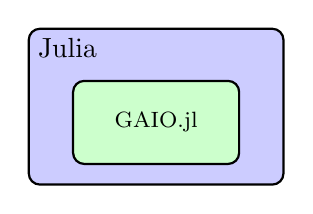
\begin{tikzpicture}[auto, node distance=2cm,>=latex']
    \node at (0,-2) [block] (julia) {\parbox{3cm}{Julia\vspace*{1.5cm}}};
    \node at (0,-2.2) [block,fill=green!20] (gaio) {{\footnotesize GAIO.jl}};
\end{tikzpicture}
    \caption{GAIO.jl architecture}
    \label{fig:arch}
\end{figure}

GAIO was fully redesigned and rebuilt in the Julia language starting in 2020. The reason to do so (and the decision to use Julia) was twofold:

\begin{enumerate}
    \item \emph{Solving the two language problem.} The set-oriented techniques require too many evaluations of the map $f$ to be reasonably implemented in an interpreted language. As with many scientific computing applications, compilation into fast machine code is necessary if one wishes to apply the methods to a non-trivial problem. However, the code should still be easy to write and read. 
    
    \item \emph{Abstraction of the syntax.} The original GAIO code required the user to be aware of the details of the internal data structures. For example, box collections were stored in a binary tree and flags in the nodes of that tree were used in order to implement the box map $F:2^\cP\to 2 ^\cP$. In Fig.~\ref{fig:attr_matlab}, we show the original GAIO/Matlab implementation of the algorithm for computing the relative global attractor in Section~\ref{sec:attractors}.
\begin{figure}[h]
\begin{lstlisting}[language=Matlab,mathescape]
function relative_attractor(tree, f, steps)
    for i = 1:steps,
        tree.set_flags('all', to_be_subdivided); 
        tree.subdivide(to_be_subdivided);   
        b = tree.boxes(-1); 
        while (~isempty(b))
            c = b(1:d); 
            r = b(d+1:2*d);
            P = X*diag(r) + ones(size(X))*diag(c); 
            tree.set_flags(f(P)$'$, hit);          
            b = tree.next_box(-1);
        end
        tree.remove(hit);                         
    end
\end{lstlisting}
\caption{Relative attractor algorithm in Matlab. Compare with Fig. \ref{fig:attr_julia}}
\label{fig:attr_matlab}
\end{figure}

In contrast, in GAIO.jl, details on how box collections are stored and how the box map $F:2^\cP\to 2 ^\cP$ is realized are essentially completely hidden from the user. After defining $F$ as a \texttt{BoxMap}, it can simply be applied to a \texttt{BoxSet}, resulting in another \texttt{BoxSet}. Since \texttt{BoxSet} is a subtype of \texttt{AbstractSet}, all set operations can be applied. As a result, the implementation of set-oriented algorithms -- like the algorithm for computing relative attractors in Fig.~\ref{fig:attr_julia} -- is very close to its mathematical formulation.

    
%    \item \emph{No longer needing to tradeoff simplicity and transparency.} The speed of a modern compiled language on today's hardware comes with an added benefit: code does not \emph{need} to be hyper-optimized - "mostly" optimized is good enough. GAIO originally used a tree data structure to represent partitions of phase space in such a way that each box was represented by a precise bitstring, maximally utilizing every byte of memory. While this was efficient, it made the data difficult to decipher. More generally, a decision always had to be made. Either
%    
%    \begin{enumerate}
%        \item complexity is hidden behind convenience functions, sacificing knowledge of "what's actually going on", or,
%        \item code is "transparent", allowing for extensibility while sacrificing clarity. 
%    \end{enumerate}
%
%    GAIO.jl was written with the knowledge that today, this just is not strictly necessary anymore. A memory-efficient tree structure is still offered, but the primary technique for partitioning phase space is much simpler: just use a grid with Cartesian indices - \emph{keep it simple, stupid}. 
\end{enumerate}


\subsection{Fitting into Julia's ecosystem}

Another reason for the decision to use Julia for GAIO.jl is the large (and growing) open source scientific computing community. GAIO.jl makes extensive use of linear algebra routines (LinearAlgebra.jl \cite{bezanson2017julia}), sparse arrays (SparseArrays.jl \cite{bezanson2017julia}, Arpack.jl \cite{arpack}), graph/network routines (MatrixNetworks.jl \cite{matrixnetworks}), and numerical integrators (DifferentialEquations.jl \cite{differentialequations}), plotting ecosystems (Makie.jl \cite{makie}, Plots.jl \cite{plots}), among others. 

A particular example of the effectiveness of such an open source scientific computing model is CUDA.jl. The sample-point methods for cell mapping are examples of so-called \emph{embarrassingly parallel} \cite{parallel} problems. It has therefore been a long-standing desire to utilize the GPU to perform such massively parallel algorithms in GAIO. However, under the previous architecture this would have to be written in CUDA's native C interface, which suffers the issues mentioned in the preceeding section. 

This is solved by the amazing work done to create CUDA.jl. The cell mapping can be written as a generic kernel whose length (in lines of code) is the same as the standard code, meaning the algorithms that make up GAIO.jl can receive up to a 200-fold \cite{gaiocuda} performance boost without ever sacrificing readability. 

Furthermore, the open-source nature of Julia's ecosystem has helped in programming GAIO.jl countless times. Since code is freely available, code reuse is common among the Julia community.

\section{Conclusion}

The Julia package GAIO.jl is introduced via an example of a three dimensional dynamical system. The software has been redesigned and rebuilt from the ground up to balance high performance and elegance, no longer needing to rely on two languages to do so. Future work is planned to use these structures e.g. for homology computation in cubical complexes, as well as to even more tightly integrate into the existing scientific computing ecosystem.
% e.g. DynamicalSystems.jl \cite{dynamicalsystemsjl,dynamicalsystemsbook} in the Julia programming language. 

\todo{fix references <- was muss geändert werden?}

\input{bib.tex}

\end{document}

% Inspired by the International Journal of Computer Applications template
